\begin{frame}{Definition}
  
  \begin{block}{Tree}
    A \emph{tree} is a graph where every pair of vertices has a path between them, and there are no cycles.
  \end{block}
  
  \begin{columns}
    \begin{column}{0.5\textwidth}
      \begin{center}
        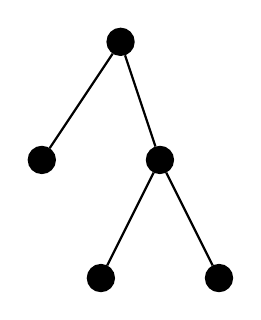
\begin{tikzpicture}
        \begin{scope}[every node/.style={circle,thick,draw,fill}]
        \node (a) at (1.5,3) {};
        \node (b) at (0.5,1.5) {};
        \node (c) at (2,1.5) {};
        \node (d) at (1.25,0) {};
        \node (e) at (2.75,0) {};
        \end{scope}
        \begin{scope}[every edge/.style={draw=black,thick}]
        \path (a) edge (b)
              (a) edge (c)
              (c) edge (d)
              (c) edge (e);
        \end{scope}
        \end{tikzpicture}
      \end{center}
    \end{column}
    \begin{column}{0.5\textwidth}
      \begin{center}
        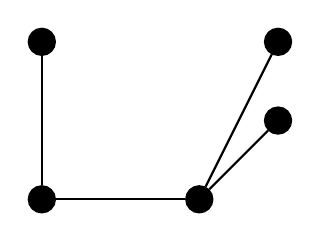
\begin{tikzpicture}
        \begin{scope}[every node/.style={circle,thick,draw,fill}]
        \node (a) at (0,3) {};
        \node (b) at (0,1) {};
        \node (c) at (2,1) {};
        \node (d) at (3,2) {};
        \node (e) at (3,3) {};
        \end{scope}
        \begin{scope}[every edge/.style={draw=black,thick}]
        \path (a) edge (b)
              (b) edge (c)
              (c) edge (d)
              (c) edge (e);
        \end{scope}
        \end{tikzpicture}
      \end{center}
    \end{column}
  \end{columns}
\end{frame}

\begin{frame}{Rooted trees}
  \begin{description}
    \item[Any vertex] of a tree can be called its root.
    \item[Levels] Root is at level 0, neighbours of the root are at level 1, their other neighbours at level 2, and so on.
    \item[Height] of a tree is $h$, where there's vertex at level $h$ but not at level $h+1$.
    \item[Leaf] Vertex at level $i$ not connected to a vertex at level $i+1$.
  \end{description}
  \begin{center}
    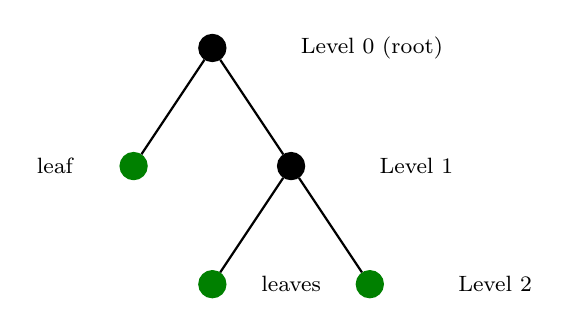
\begin{tikzpicture}
    \begin{scope}[every node/.style={circle,thick,draw,fill}]
      \node (a) at (1.5,3 ) {};
      \node (b)[green!50!black] at (0.5,1.5) {};
      \node (c) at (2.5,1.5) {};
      \node (d)[green!50!black] at (1.5,0) {};
      \node (e)[green!50!black] at (3.5,0) {};
    \end{scope}
    \node () [right of=a, anchor=west] {\footnotesize Level 0 (root)};
    \node () [right of=c, anchor=west] {\footnotesize Level 1};
    \node () [right of=e, anchor=west] {\footnotesize Level 2};
    \node () [left of=b] {\footnotesize leaf};
    \node () [left of=e] {\footnotesize leaves};
    \begin{scope}[every edge/.style={draw=black,thick}]
      \path (a) edge (b)
            (a) edge (c)
            (c) edge (d)
            (c) edge (e);
    \end{scope}
    \end{tikzpicture}
  \end{center}
\end{frame}

\begin{frame}{$m$-ary Rooted Tree}
  \begin{definition}
    When a vertex at level $i$ is connected to a vertex at level $i+1$ it's common to call the former the \emph{parent} and the latter the \emph{child}.
    A rooted tree is $m$-ary if every parent has the same number of children.
    A $2$-ary rooted tree is called a \emph{binary tree}.
  \end{definition}
  \begin{center}
    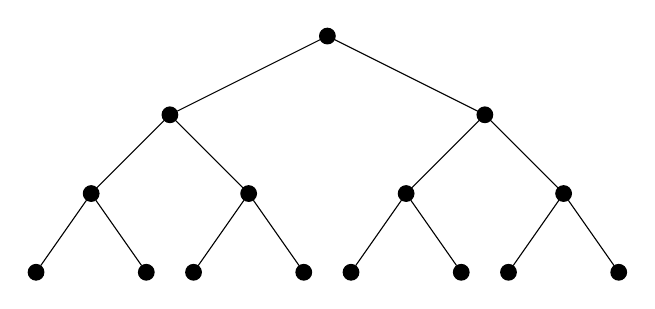
\begin{tikzpicture}
    \begin{scope}[every node/.style={circle,draw,fill,scale=0.6}]
    \node (a) at (3,4) {};
    \node (b) at (1,3) {};
    \node (c) at (5,3) {};
    \node (d) at (0,2) {};
    \node (e) at (2,2) {};
    \node (f) at (4,2) {};
    \node (g) at (6,2) {};
    \node (h) at (-0.7,1) {};
    \node (i) at (0.7,1) {};
    \node (j) at (1.3,1) {};
    \node (k) at (2.7,1) {};
    \node (l) at (3.3,1) {};
    \node (m) at (4.7,1) {};
    \node (n) at (5.3,1) {};
    \node (o) at (6.7,1) {};
    \end{scope}
    \begin{scope}[every edge/.style={draw=black}]
    \path (a) edge (b)
          (a) edge (c)
          (b) edge (d)
          (b) edge (e)
          (c) edge (f)
          (c) edge (g)
          (d) edge (h)
          (d) edge (i)
          (e) edge (j)
          (e) edge (k)
          (f) edge (l)
          (f) edge (m)
          (g) edge (n)
          (g) edge (o);
    \end{scope}
    \end{tikzpicture}
  \end{center}
\end{frame}

\begin{frame}[fragile]{Isomorphic Rooted Trees}
  \begin{definition}
   Two rooted trees are said to be \emph{isomorphic} if there is a graph isomorphism between them which takes the root of one tree to the root of the other.
  \end{definition}
  \vspace{5mm}
  \begin{columns}
    \begin{column}{0.4\textwidth}
      \begin{center}
        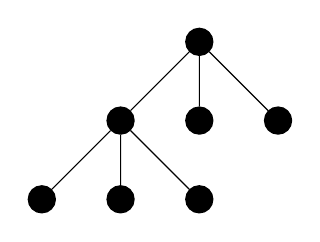
\begin{tikzpicture}[level/.style={level distance = 1cm},level 1/.style={sibling distance=10mm},level 2/.style={sibling distance=10mm}]
          \begin{scope}[every node/.style={circle,thick,draw,fill}]
            \node {}
              child { node {}
                child { node {} }
                child { node {} }
                child { node {} }
              }
              child { node {}
              }
              child { node {}
              };
          \end{scope}
        \end{tikzpicture}
      \end{center}
    \end{column}
    \begin{column}{0.4\textwidth}
      \begin{center}
        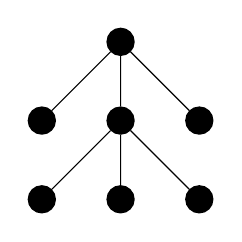
\begin{tikzpicture}[level/.style={level distance = 1cm},level 1/.style={sibling distance=10mm},level 2/.style={sibling distance=10mm}]
          \begin{scope}[every node/.style={circle,thick,draw,fill}]
            \node {}
              child { node {}
              }
              child { node {}
                child { node {} }
                child { node {} }
                child { node {} }
              }
              child { node {}
              };
          \end{scope}
        \end{tikzpicture}
      \end{center}
    \end{column}
  \end{columns}
\end{frame}

\begin{frame}{Logarithms}
  We define $\log$ in the following way:
  \[ m^h = l \Leftrightarrow \log_m l = h \]

  \begin{alertblock}{What does $log$ mean?}
    Suppose we have two numbers $m$ and $h$ and we ask the question ``what is $m$ to the power of $h$?''
    Let's call the answer $l$, so $l = m^h$.

    The $\log$ function asks the inverse question: ``what do we need to raise $m$ to the power of to get $l$?''
    The answer is $h$.

    For example, $10^2 = 100$ so $\log_{10} 100 = 2$.
    The subscript $10$ is called the \emph{base}.
  \end{alertblock}
\end{frame}

\begin{frame}{Heights and leaves of $m$-ary rooted trees}
  \begin{theorem}
    The height $h$ of an $m$-ary rooted tree with $l$ leaves is at least $\log_m l$.
    That is: $h \geq \log_m l$.
  \end{theorem}
  \begin{proof}
    Note that $h \geq log_m l \hspace{0.1cm} \Leftrightarrow \hspace{0.1cm} m^h \geq m^{log_m l} \hspace{0.1cm} \Leftrightarrow \hspace{0.1cm} m^h \geq l$.
    So, just show that $l$ is at most $m^h$.
    
    For a tree of height 0, $m^0 = 1$ and $l=0$ giving $m^h = l$.
    Next, assume trees of height $i-1$ have at most $m^{i-1}$ leaves.
    From a tree of height $i$, we can create $m$ trees of height at most $i-1$ by deleting the root.
    Each of these smaller trees has at most $m^{i-1}$ leaves.
    So, the big tree has at most $m \times m^{i-1} = m^i$ leaves.
  \end{proof}
\end{frame}

\begin{frame}[fragile]{Examples of heights and leaves of $m$-ary trees}
  \begin{columns}
    \begin{column}{0.5\textwidth}
      \begin{center}
        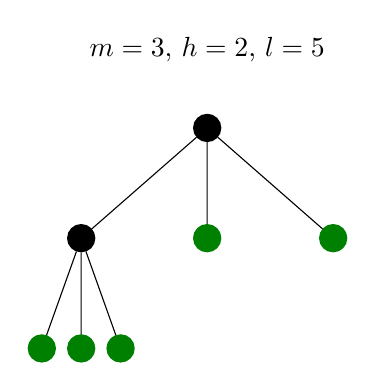
\begin{tikzpicture}[level/.style={level distance = 1.4cm},level 1/.style={sibling distance=16mm},level 2/.style={sibling distance=5mm}]
          \begin{scope}[every node/.style={circle,thick,draw,fill}]
            \node {}
              child { node {}
                child { node[green!50!black] {} }
                child { node[green!50!black] {} }
                child { node[green!50!black] {} }
              }
              child { node[green!50!black] {}
              }
              child { node[green!50!black] {}
              };
          \end{scope}
          \node at (0,1) {$m=3$, $h=2$, $l=5$};
        \end{tikzpicture}
      \end{center}
    \end{column}
    \begin{column}{0.5\textwidth}
      \begin{center}
        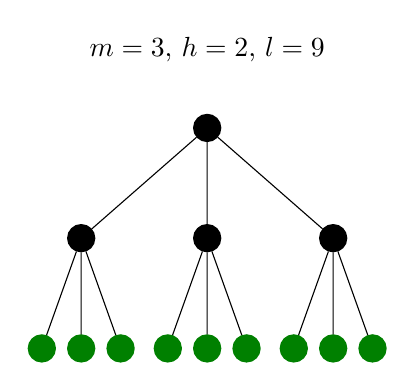
\begin{tikzpicture}[level/.style={level distance = 1.4cm},level 1/.style={sibling distance=16mm},level 2/.style={sibling distance=5mm}]
          \begin{scope}[every node/.style={circle,thick,draw,fill}]
            \node {}
              child { node {}
                child { node[green!50!black] {} }
                child { node[green!50!black] {} }
                child { node[green!50!black] {} }
              }
              child { node {}
                child { node[green!50!black] {} }
                child { node[green!50!black] {} }
                child { node[green!50!black] {} }
              }
              child { node {}
                child { node[green!50!black] {} }
                child { node[green!50!black] {} }
                child { node[green!50!black] {} }
              };
          \end{scope}
          \node at (0,1) {$m=3$, $h=2$, $l=9$};
        \end{tikzpicture}
      \end{center}
    \end{column}
  \end{columns}
\end{frame}


\begin{frame}[fragile]{Deleting the root of an $m$-ary tree}
  \begin{center}
    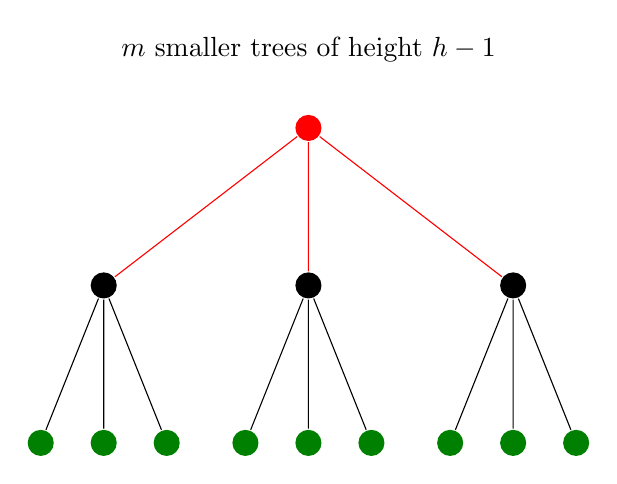
\begin{tikzpicture}[level/.style={level distance = 2cm},level 1/.style={sibling distance=26mm},level 2/.style={sibling distance=8mm}]
      \begin{scope}[every node/.style={circle,thick,fill}]
        \node[fill=red] {}
          child[draw=red] { node {}
            child[draw=black] { node[green!50!black] {} }
            child[draw=black] { node[green!50!black] {} }
            child[draw=black] { node[green!50!black] {} }
          }
          child[draw=red] { node {}
            child[draw=black] { node[green!50!black] {} }
            child[draw=black] { node[green!50!black] {} }
            child[draw=black] { node[green!50!black] {} }
          }
          child[draw=red] { node {}
            child[draw=black] { node[green!50!black] {} }
            child[draw=black] { node[green!50!black] {} }
            child[draw=black] { node[green!50!black] {} }
          };
      \end{scope}
      \node at (0,1) {$m$ smaller trees of height $h-1$};
    \end{tikzpicture}
  \end{center}
\end{frame}





\begin{frame}{Spanning trees}
  \begin{alertblock}{Subgraph}
    A \emph{subgraph} $H = (V_H, E_H)$ of a graph $G = (V,E)$ is a graph such that $V_H$ is a subset of $V$, $E_H$ is a subset of $E$, and no edge in $E_H$ contains a vertex not in $V_H$.
  \end{alertblock}
  \vspace{0.4cm}
  \begin{alertblock}{Spanning Tree}
    A \emph{spanning tree} $T$ of a connected graph $G$ is a subgraph of $G$ such that:
    \begin{itemize}
      \item the vertex set of $T$ is the vertex set of $G$ and
      \item $T$ is a tree.
    \end{itemize}
  \end{alertblock}
\end{frame}

\begin{frame}[fragile]{Spanning tree example}
  \begin{center}
    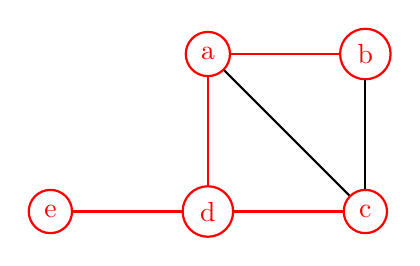
\begin{tikzpicture}
      \begin{scope}[every node/.style={circle,thick,draw=red,text=red}]
        \node (a) at (2,2) {a};
        \node (b) at (4,2) {b};
        \node (c) at (4,0) {c};
        \node (d) at (2,0) {d};
        \node (e) at (0,0) {e};
      \end{scope}
      \begin{scope}[every edge/.style={draw=red,thick}]
        \path (a) edge (b);
        \path (a) edge[draw=black] (c);
        \path (a) edge (d);
        \path (b) edge[draw=black] (c);
        \path (c) edge (d);
        \path (d) edge (e);
      \end{scope}
    \end{tikzpicture}
  \end{center}
  \begin{center}
    Spanning tree in red.
  \end{center}
\end{frame}